\chapter{sed}
\label{chap:sed}

Sed\index{sed}是一个超级流式编辑器。
picture a stream flowing through a pipe. Okay, you can't see a stream
if it's inside a pipe. That's what I get for attempting a flowing
analogy. You want literature, read James Joyce.

Anyhow, sed is a marvelous utility. Unfortunately, most people never
learn its real power. The language is very simple, but the
documentation is terrible. The Solaris on-line manual pages for sed
are five pages long, and two of those pages describe the 34 different
errors you can get. A program that spends as much space documenting
the errors than it does documenting the language has a serious
learning curve.

Do not fret! It is not your fault you don't understand sed. I will
cover sed completely. But I will describe the features in the order
that I learned them. I didn't learn everything at once. You don't need
to either.

sed的工作流程:
\begin{figure}[!htbp]
  \centering
  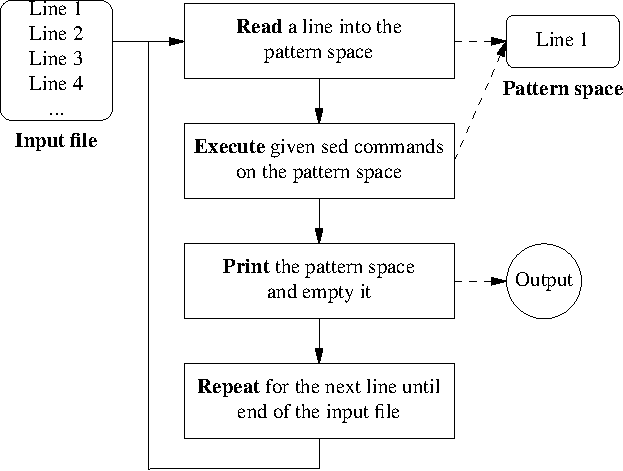
\includegraphics[width=.65\textwidth]{graph/sed_workflow.pdf}
    \caption{sed工作流程}
  \label{fig:sed_workflow}
\end{figure}

命令列表:

\begin{tabular}{lp{25em}}
\toprule
命令       & 说明 \\
\midrule
a          & 在当前行后面追加文本 \\
b label    & 分支到脚本中带有标号的地方,如果标号不存在就分支到脚本的末尾 \\
c          & 用新的文本改变或者替代本行的文本 \\
d          & 从模板块(Pattern space)位置删除行 \\
D          & 删除模板块的第一行 \\
i          & 在当前行上面插入文本 \\
h          & 拷贝模板块的内容到内存中的缓冲区 \\
H          & 追加模板块的内容到内存中的缓冲区 \\
g          & 获得内存缓冲区的内容,并替代当前模板块中的文本 \\
G          & 获得内存缓冲区的内容,并追加到当前模板块文本的后面 \\
l          & 列表不能打印字符的清单 \\
n          & 读取下一个输入行,用下一个命令处理新的行而不是用第一个命令 \\
N          & 追加下一个输入行到模板块后面并在二者之间嵌入一个新的行,改变当前行的号码 \\
p          & 打印模板块的行 \\
P          & 打印模板块的第一行 \\
q          & 退出 sed \\
r file     & 从file中读行 \\
t label    & if分支,从最后一行开始,条件一旦被满足或者T命令或者t命令, 将导致分支到带有标号的命令处,或者到脚本的末尾 \\
T label    & 错误分支,从最后一行开始,一旦发生错误或者T命令或者t命令, 将导致分支到带有标号的命令处,或者到脚本的末尾 \\
w file     & 写并追模板块到file末尾 \\
W file     & 写并追模板块的第一行到file末尾 \\
!          & 表示后面的命令对所有没有被选定的行发生作用 \\
s/re/string/ & 用string替换正则表达式re \\
=          & 打印当前行号码 \\
注释command & 把注释扩展到下一个换行符以前替换标记 \\
g           & 行内全面替换 \\
p           & 打印行 \\
w           & 把行写入一个文件 \\
x           & 互换模板块中的文本和缓冲区中的文本 \\
y           & 把一个字符翻译为另外的字符(但是不能用于正则表达式) \\
\bottomrule
\end{tabular}

一些选项:

\begin{tabular}{l|lp{20em}}
\hline
-e command             & 允许多点编辑 \\
\hline
--expression=command   & 同上 \\
\hline
-h,--help              & 打印命令行选项摘要,并显示 bug 列表的地址 \\
\hline
-n,--quiet,--silent    & 取消默认输出 \\
\hline
-f,                    & 引导 sed 脚本文件名 \\
\hline
--filr=script-file     & 同上 \\
\hline
-V,--version           & 打印版本和版权信息\\
\hline
\end{tabular}

\section{匹配}
\label{sec:sedPattern}

\subsection{变量定义}
\label{subsec:sedVariableDef}

\section{特殊变量}
\label{sec:sedSpecialVariable}

\section{数组}
\label{sec:sedArray}

\section{删除}
\label{sec:sedDelete}

删除(d)编辑命令采用一个地址,如果行匹配这个地址就删除模式空间的内容。
删除命令(d)还是一个可以改变脚本中的控制流的命令。这是因为一旦执行这个
命令,那么在“空的”模式空间中就不会再有命令执行。删除命令(d)会导致读取
新输入行,而编辑脚本则从头开始新的一轮。重要的是,如果某行匹配这个地址,
那么就删除整个行,而不只是删除行中匹配的部分。

\section{替换}
 
Sed有众多命令,但经常被用到的就是最基本的替换命令“s”了, 替换命令有四部
分组成,如下表所示:

\begin{table}[h]
\centering
\begin{tabular}{l|l}
\hline
s	     & 所使用的命令是替换命令 \\
\hline
/../../	 & 所使用的分隔符,可以自行改变,不过三个符号要一致 \\
\hline
old	     & 这是将要被替换的字符串或正则表达式 \\
\hline
new	     & 这是替换后的字符串 \\
\hline
\end{tabular}
\end{table}

sed s/day/night/ <old >new

eg: sed 's/local/host/[g]' /etc/hosts
 
Or another way (for Unix beginners), 

sed s/day/night/ old >new
 
我们也可以如下这样写,

\small{
\begin{verbatim}
echo day | sed s/day/night/ 
\end{verbatim}
}
\normalsize

将会输出“night”。

我们在这里并没有使用引号把这些参数给引用起来,也能得出想要的结果,因为
这个例子是不需要它们的,嘿嘿!然而,在使用过程中出现了原字符,这时候引
号是必须要的。如果我们不确定何时要使用引号,那么,最好的习惯就是“每用
必带”引号即可,不用纠结那么多。

sed 's/day/night/' <old >new

I must emphasize that the sed editor changes exactly what you tell it
to. So if you executed
 
\begin{verbatim}
eg: # echo Sunday | sed 's/day/night/'
output: Sunnight
\end{verbatim}
 
This would output the word "Sunnight" bacause sed found the string
"day" in the input.
 
The search pattern is on the left hand side and the replacement string
is on the right hand side.
 
We've covered quoting and regular expressions. That's 90\% of the
effort needed to learn the substitute command. To put it another way,
you already know how to handle 90\% of the most frequent uses of
sed. There are a ... few fine points that an future sed expert should
know about. (You just finished section 1. There's only 63 more
sections to cover. :-) Oh. And you may want to bookmark this page,
.... just in case you don't finish.

\section{追加、插入和更改}
\label{sec:appendInsertChange}

追加(a)、更改(c)、插入(i)编辑命令提供了类似于vi交互式编辑器的编辑功能。

追加命令(a)将文本放置在当前行之后。更改命令(c)用所指定的文本取代模
式空间的内容。插入命令(i)将所提供的文本放置在模式空间的当前行之前。这
些命令中的每一个都要求后面跟一个反斜杠用于转义第一个行尾。如要输入多行
文本,每个连续的行都必须用反斜杠结束,最后一行除外。而且,如果文本包含
一个字面含义的反斜杠,要再添加一个反斜杠来转义它。

\section{模式空间和保留空间}
\label{sec:patternSpace}

\section{流控制}
\label{sec:flowControl}

\section{地址范围}
\label{sec:addrSpace}

\section{调用外部变量}
\label{sec:callExternalVariable}

\section{总结}
\label{sec:summary}

